%! Author = lili
%! Date = 8/1/26


\section{Divide-and-Conquer Alignment}\label{sec:divide-and-conquer-alignment}
\skript{In this section we present a heuristic for sum-of-pairs multiple sequence alignment that no longer
gives any guarantee about the resulting alignment cost, although in practice it is often very good.
Therefore, the method is a \emph{correctness heuristic}. While in the worst case the running time is
still exponential in the number of sequences, the advantages are a polynomial space usage and that on
average the practical running time is much faster than the exhaustive search, while the result is very
often still optimal or close to optimal.}

\begin{idee}
    \skript{The basic idea of the heuristic is to cut all sequences at suitable cut points into left and right
    parts, and then to solve the two such generated alignment problems for the left parts and the right
    parts separately. This is done either by recursion or, if the sequences are short enough, by an exact
    algorithm. For a graphical sketch of the procedure.} % TODO , see Figure~10.1.
\end{idee}

\paragraph{Finding cut positions.} \skript{The main question about this procedure is how to choose good cut positions, since this choice is
obviously critical for the quality of the final alignment. The ideal case is easy to formulate:}

\defin{optimal_cut}

\skript{There are many optimal cut positions, e.g.\ the trivial ones $(0, 0, \ldots, 0)$ and $(n_1, n_2,
\ldots, n_k)$. In fact:}

\begin{lem}
    \skript{For any cut position $\hat c_1\in\{0, \ldots, n_1\}$ of the first sequence $s_1$, there exist cut
    positions $c_2, \ldots, c_k$ of the remaining sequences $s_2, \ldots, s_k$ such that $(\hat c_1, c_2,
    \ldots, c_k)$ is an optimal cut of the sequences $s_1, s_2, \ldots, s_k$.
    \paragraph{Proof}
    Assume that $A^{\mathrm{opt}}$ is an optimal alignment. Choose one of the points between the characters
    in the first row of $A^{\mathrm{opt}}$ that correspond to the characters $s_1[\hat c_1]$ and
        $s_1[\hat c_1+1]$. The vertical ``cut'' at this point through the optimal alignment defines the cut
        positions $c_2, \ldots, c_k$ that, together with $\hat c_1$, are optimal by definition. See Figure~10.2
        for an illustration.
    }
\end{lem}

% TODO \caption{Overview of divide-and-conquer multiple sequence alignment.}

% TODO \caption{Connection between unaligned sequences $s_1,\ldots,s_k$ (left) and a multiple alignment $A$ of
%them (right). If $A$ is an optimal alignment $A^{\mathrm{opt}}$, any vertical cut in the alignment
%corresponds to an optimal cut of the sequences.}

\skript{
    The lemma tells us that a first cut position $\hat c_1$ of $s_1$ can be chosen arbitrarily (for
    symmetry reasons and to arrive at an efficient divide-and-conquer procedure, we will use $\hat c_1 =
    \lceil n_1/2\rceil$), and then there always exist cut positions of the other sequences that produce an
    optimal cut.

    The NP-completeness of the SP-alignment problem implies, however, that it is unlikely that there exists
    a polynomial time algorithm for finding optimal cuts of this type. Hence a heuristic is used to find
    good, though not always optimal cut positions.

    This heuristic is based on pairwise sequence comparisons whose results are stored in an additional cost
    matrix that contains for each pair of cut positions $(c_p, c_q)$ the penalty (additional cost) imposed
    by cutting the two sequences at these points, instead of cutting them at points compatible with an
    optimal pairwise alignment (see Definition~\ref{def:additional_cost_matrix}). The efficient computation of additional cost matrices
    was discussed in Section~\ref{sec:the-forward-backward-technique}.

    The idea of using additional cost matrices to quantify the quality of a family of cut positions is that
    the closer a potential cut point is to an optimal pairwise alignment path, the smaller will be the
    contribution of this pair to the overall sum-of-pairs multiple alignment cost. Since we are dealing
    with sum-of-pairs alignment, we define the additional cost of a family of cuts along the same rationale.}

\deffin{multiple_additional_cost}

\skript{Although maybe unintuitive, even a family of cut positions with zero multiple additional cost, i.e.\ one
whose implied pairwise cuts are all compatible with the corresponding pairwise optimal alignments, is
not necessarily optimal (see Example~\ref{bsp:multiple_additional_cost}). The converse is also not true: Neither has an optimal cut
always multiple additional cost zero, nor is a cut with smallest possible additional cost necessarily
optimal.}

\begin{bsp}
    \label{bsp:multiple_additional_cost}
    \skript{
        Let $s_1 = \mathtt{CT}$, $s_2 = \mathtt{AGT}$, and $s_3 = \mathtt{G}$. Using unit cost edit distance, the
        three additional cost matrices are the following:
        \[
            C_{(1,2)}:\
            \begin{array}{c|cccc}
                & \epsilon & \mathtt{A} & \mathtt{G} & \mathtt{T}\\\hline
                \epsilon & 0 & 0 & 1 & 3\\
                \mathtt{C} & 1 & 0 & 0 & 2\\
                \mathtt{T} & 3 & 2 & 1 & 0
            \end{array}
            \quad
            C_{(1,3)}:\
            \begin{array}{c|cc}
                & \epsilon & \mathtt{G}\\\hline
                \epsilon & 0 & 1\\
                \mathtt{C} & 0 & 0\\
                \mathtt{T} & 1 & 0
            \end{array}
            \quad
            C_{(2,3)}:\
            \begin{array}{c|cc}
                & \epsilon & \mathtt{G}\\\hline
                \epsilon & 0 & 2\\
                \mathtt{A} & 0 & 1\\
                \mathtt{G} & 1 & 0\\
                \mathtt{T} & 2 & 0
            \end{array}
        \]
        There are two cuts $(1,1,0)$ and $(1,2,1)$, both of which yield a multiple additional cost
        $C(1,1,0) = C(1,2,1) = 0$. Nevertheless, the implied multiple alignments are not necessarily optimal as
        can be seen for the cut $(1,1,0)$:
        \[
            \begin{array}{c|c}
                \mathtt{C} & \mathtt{T}\\
                \mathtt{A} & \mathtt{GT}\\
                \varepsilon & \mathtt{G}
            \end{array}
            \to
            \begin{pmatrix}
                \mathtt{C}\\\mathtt{A}\\\mathtt{-}
            \end{pmatrix}
            ++
            \begin{pmatrix}
                \mathtt{-}&\mathtt{T}\\\mathtt{G}&\mathtt{T}\\\mathtt{G}&\mathtt{-}
            \end{pmatrix}
            =
            \begin{pmatrix}
                \mathtt{C}&\mathtt{-}&\mathtt{T}\\\mathtt{A}&\mathtt{G}&\mathtt{T}\\
                \mathtt{-}&\mathtt{G}&\mathtt{-}
            \end{pmatrix}
            \ \text{(SP-cost 7, not optimal).}
        \]
        But they might be optimal, as for the cut $(1,2,1)$:
        \[
            \begin{array}{c|c}
                \mathtt{C} & \mathtt{T}\\
                \mathtt{AG} & \mathtt{T}\\
                \mathtt{G} & \varepsilon
            \end{array}
            \to
            \begin{pmatrix}
                \mathtt{-}&\mathtt{C}\\\mathtt{A}&\mathtt{G}\\\mathtt{-}&\mathtt{G}
            \end{pmatrix}
            ++
            \begin{pmatrix}
                \mathtt{T}\\\mathtt{T}\\\mathtt{-}
            \end{pmatrix}
            =
            \begin{pmatrix}
                \mathtt{-}&\mathtt{C}&\mathtt{T}\\\mathtt{A}&\mathtt{G}&\mathtt{T}\\
                \mathtt{-}&\mathtt{G}&\mathtt{-}
            \end{pmatrix}
            \ \text{(SP-cost 6, optimal).}
        \]}
\end{bsp}

\skript{Nevertheless, it is a good heuristic to choose cuts minimizing the multiple additional cost.}

\paragraph{DCA Algorithm.} \skript{The divide-and-conquer alignment algorithm first chooses an arbitrary cut position $\hat c_1$ for the
first sequence (usually the sequence is cut in half for symmetry reasons) and then searches for the
remaining cut positions $c_2, \ldots, c_k$ such that the cut $(\hat c_1, c_2, \ldots, c_k)$ minimizes
    $C(\hat c_1, c_2, \ldots, c_k)$.

    Then the sequences are cut in this way, and the procedure is repeated recursively until the maximal
    sequence length drops below a threshold value $L$, when an exact multiple sequence alignment algorithm
    MSA (e.g.\ using Carrillo-Lipman bounds) is applied.

    The pseudocode for this procedure is given in Algorithm~4 where $+\!\!+$ is the operator concatenating
    two alignments.}

\begin{algorithm}[H]
    \caption{$\mathrm{DCA}(s_1,s_2,\ldots,s_k;L)$}
    \label{alg:dca}
    \begin{algorithmic}[1]

        \For{$p\gets 1$ to $k$}
            \State $n_p\gets |s_p|$
        \EndFor

        \If{$\max\{n_1,n_2,\ldots,n_k\}\le L$}
            \State \Return $\mathrm{MSA}(s_1,s_2,\ldots,s_k)$
        \Else
            \State $\hat{c}_1\gets\lceil n_1/2\rceil$
            \State Compute $(c_2,\ldots,c_k)$ such that
            $C(\hat{c}_1,c_2,\ldots,c_k)$ is minimum
            \State \Return
            $\mathrm{DCA}(s_1[1\ldots\hat{c}_1],
            s_2[1\ldots c_2],\ldots,
            s_k[1\ldots c_k];L)$
            \Statex \hspace{1cm}$++\
            \mathrm{DCA}(s_1[\hat{c}_1+1\ldots n_1],
            s_2[c_2+1\ldots n_2],\ldots,
            s_k[c_k+1\ldots n_k];L)$
        \EndIf
    \end{algorithmic}
\end{algorithm}

\skript{The search space in the computation of cut positions is sketched in Figure~10.3. % TODO
Since the cut position
of the first sequence $s_1$ is fixed to $\hat c_1$ but the others can vary over their whole sequence
length, the search space has size $O(n_2\cdot n_3\cdots n_k)$. This implies that the time for computing
a cut (i.e., finding the minimum in this search space) by exhaustive search takes $O(k^2 n^2 +
n^{k-1})$ time and uses $O(k^2 n^2)$ space.}

% TODO \caption{Calculation of cut positions minimizing the multiple additional cost.}

\paragraph{Overall complexity.}
\skript{
    Let $L$ be the length bound below which the exact MSA algorithm is applied. Assuming that the maximum
    sequence length $n$ is of the form $n = L\cdot 2^D$ and all cuts are symmetric (i.e., $n_{(d)} = n/2^d$
    for all $d = 0, \ldots, D-1$), the whole divide-and-conquer alignment procedure has the overall time
    complexity
    \[
        \begin{aligned}
            &\left(\sum_{d=0}^{D-1} 2^d\Bigl(k^2 n_{(d)}^2 + n_{(d)}^{k-1}\Bigr)\right) + \frac{n}{L}\bigl(2^k
            L^{k-1} k^2\bigr)\\
            &= \left(\sum_{d=0}^{D-1} 2^d\Bigl(k^2\frac{n^2}{2^{2d}} + \frac{n^{k-1}}{2^{d(k-1)}}\Bigr)\right) +
            2^k n L^{k-1} k^2\\
            &= \left(\sum_{d=0}^{D-1}\Bigl(k^2\frac{n^2}{2^d} + \frac{n^{k-1}}{2^{d(k-2)}}\Bigr)\right) + 2^k n
            L^{k-1} k^2\\
            &\le \left(\sum_{d=0}^{D-1}\Bigl(k^2\frac{n^2}{2^d} + \frac{n^{k-1}}{2^d}\Bigr)\right) + 2^k n L^{k-1}
            k^2 && \text{(since } k\ge 3)\\
            &= \bigl(k^2 n^2 + n^{k-1}\bigr)\left(\sum_{d=0}^{D-1}\frac{1}{2^d}\right) + 2^k n L^{k-1} k^2\\
            &\le \bigl(k^2 n^2 + n^{k-1}\bigr)\cdot 2 + 2^k n L^{k-1} k^2 && \text{(geometric series)}\\
            &\in O\bigl(k^2 n^2 + n^{k-1} + 2^k n L^{k-1} k^2\bigr)
        \end{aligned}
    \]
    and space complexity
    \[
        \max_{0\le d<D}\left( k n_{(d)} + \binom{k-1}{2} n_{(d)}^2\right) + L^k \in O\bigl(k^2 n^2 + L^k\bigr).
    \]

    Compared to the standard dynamic programming for multiple alignment, the time is reduced only by one
    dimension, so it is not clear if the whole method is really an advantage. However:
    \begin{itemize}
        \item The space usage for the whole divide-and-conquer alignment procedure can be seen as polynomial
        since the space is mainly required for the $\binom{k}{2}$ additional cost matrices. The exponential term
        in the space complexity to compute the exact multiple alignment for sequences shorter than $L$ can be
        neglected because $L$ is small and can be chosen freely.
        \item Additional cost matrices have a very nice structure, since the low values that are of interest
        here are often close to the main diagonal, and the values increase rapidly when one leaves this
        diagonal. Based on this observation, several branch-and-bound heuristics have been developed to speed up
        the search for good cut positions, for more details see (Stoye, 1998).
    \end{itemize}

    An implementation of the divide-and-conquer alignment algorithm, plus further documentation, can be
    found at \url{https://bibiserv.cebitec.uni-bielefeld.de/dca}.}


\section{Segment-Based Alignment}\label{sec:segment-based-alignment}
\skript{The global multiple alignment methods mentioned so far, like the progressive methods or the
simultaneous method DCA, have properties that are not necessarily desirable in all applications.

In particular, the alignment depends on many parameters, like the cost function or substitution matrix,
    gap penalties, and a scoring function (e.g.\ sum of pairs) for the multiple alignment. Apart from the
    problem that these parameters need to be chosen in advance, the global methods have the well-known
    weakness that local similarities may be aligned in a wrong way if they are not significant in a global
    context.}

\begin{bsp}[Potential misalignment that may be caused by the choice of
the affine gap penalties (Skript)]
    \[
        A = \begin{pmatrix}
                \mathtt{A}&\mathtt{F}&\mathtt{A}&\mathtt{T}&\mathtt{C}&\mathtt{A}&\mathtt{T}&
                \mathtt{C}&\mathtt{A}\\
                \mathtt{A}&\mathtt{C}&\mathtt{A}&\mathtt{T}&\mathtt{-}&\mathtt{-}&\mathtt{-}&\mathtt{-}&\mathtt{A}
        \end{pmatrix}.
    \]
    If instead of individual positions, whole units of local similarities are compared and used to build a
    global multiple alignment, the result will depend much less on the particular alignment parameters, and
    instead reflect more the local similarities in the data, like in the following example:
    \[
        A' = \begin{pmatrix}
                 \mathtt{A}&\mathtt{F}&\mathtt{A}&\mathtt{T}&\mathtt{C}&\mathtt{A}&\mathtt{T}&
                 \mathtt{C}&\mathtt{A}\\
                 \mathtt{A}&\mathtt{-}&\mathtt{-}&\mathtt{-}&\mathtt{C}&\mathtt{A}&\mathtt{T}&\mathtt{-}&\mathtt{A}
        \end{pmatrix}.
    \]
    This is the idea of segment-based sequence alignment.
\end{bsp}

\subsection{Segment Identification}\label{subsec:segment-identification}
\skript{The first step in a segment-based alignment approach is to identify the segments. There are different
possibilities to obtain segments.

The possibly simplest strategy, followed by the program TWOALIGN (Abdedda\"im, 1997) is to use
    (suboptimal) local alignments like they are computed by the Smith-Waterman or Waterman-Eggert
    algorithms. A disadvantage of this approach is that the local alignment computation also requires the
    usual alignment parameters like score function and gap penalties.

    An alternative approach is to use \emph{gap-free} local alignments. In this case, the segments
    correspond to diagonal segments of the alignment matrix. Since gap-free alignments can be computed
    faster than gapped alignments, more time can be spent on the computation of their score. The approach
    followed in the DIALIGN method (Section~\ref{subsec:dialign}) is to use a statistical objective function that assigns
    the score $P_D(l_D, s_D)$ to a diagonal $D$ of length $l_D$ with $s_D$ matches.}

\definSB{p_value_diagonal}

where $p = 0.25$ for nucleotides and $p = 0.05$ for amino acids.

\definSB{weight_diagonal}

\skript{The time to compute all diagonals is $O(n^3)$, but this can be reduced to $O(n^2)$ if the maximal
length of a diagonal segment is bounded by a constant.}

\subsection{Segment Selection and Assembly}\label{subsec:segment-selection-and-assembly}

\skript{
    After a set of segments is identified, it is not necessarily possible to assemble them into a global
    alignment, since they might be \emph{inconsistent}, i.e., the inclusion of some of the segments does not
    allow the inclusion of other segments into the alignment. In the case of two sequences, this is the
    case if and only if two segments ``cross'' as the two segments ``ON'' and ``ANA''.} % TODO  shown in Figure~10.4.

\begin{figure}

    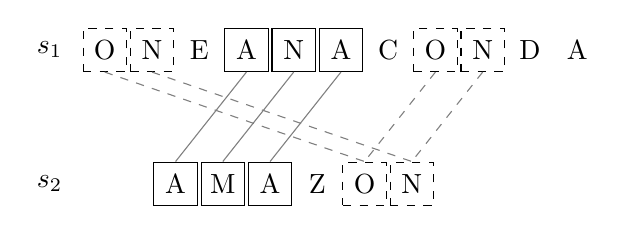
\begin{tikzpicture}[
        b/.style ={draw, minimum size=5.5mm, inner sep=0pt},
        db/.style={b, dashed}]
        \node at (-0.7,0){$s_1$};
        \foreach \l [count=\i from 0] in {O,N}      {\node[db]  (a\i) at (\i*0.6,0){\l};}
        \node  (a2) at (2*0.6,0){E};
        \foreach \l [count=\i from 3] in {A,N,A}      {\node[b]  (a\i) at (\i*0.6,0){\l};}
        \node (a6) at (6*0.6,0){C};
        \foreach \l [count=\i from 7] in {O,N}      {\node[db] (a\i) at (\i*0.6,0){\l};}
        \foreach \l [count=\i from 9] in {D,A}        {\node     (a\i) at (\i*0.6,0){\l};}
        \node at (-0.7,-1.7){$s_2$};
        \foreach \l [count=\j from 0] in {A,M,A}    {\node[b]  (b\j) at (\j*0.6+0.9,-1.7){\l};}
        \node (b3) at (3*0.6+0.9,-1.7){Z};
        \foreach \l [count=\j from 4] in {O,N}        {\node[db] (b\j) at (\j*0.6+0.9,-1.7){\l};}
% Zuordnungen (durchgezogen = Match-Lauf ANA, gestrichelt = ON)
        \draw[gray]        (a3.south) -- (b0.north);
        \draw[gray]        (a4.south) -- (b1.north);
        \draw[gray]        (a5.south) -- (b2.north);
        \draw[gray,dashed] (a7.south) -- (b4.north);
        \draw[gray,dashed] (a8.south) -- (b5.north);
        \draw[gray,dashed] (a0.south) -- (b4.north);
        \draw[gray,dashed] (a1.south) -- (b5.north);
    \end{tikzpicture}
    \space{1cm}
    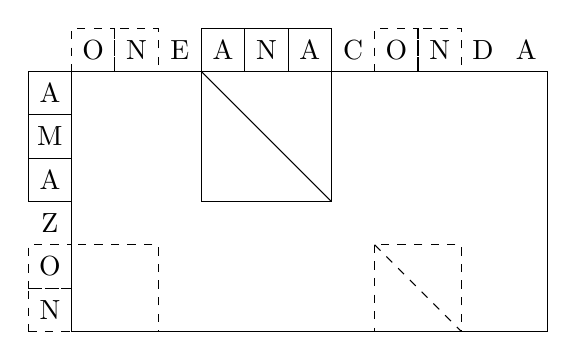
\begin{tikzpicture}[x=0.55cm, y=0.55cm, b/.style ={draw, minimum size=5.5mm, inner sep=0pt},
        db/.style={b, dashed}]
        % Spaltenkopf ONEANACONDA
        \foreach \l [count=\i from 0] in {O,N}      {\node[db]  (a\i) at (\i,1){\l};}
        \node  (a2) at (2,1){E};
        \foreach \l [count=\i from 3] in {A,N,A}      {\node[b]  (a\i) at (\i,1){\l};}
        \node (a6) at (6,1){C};
        \foreach \l [count=\i from 7] in {O,N}      {\node[db] (a\i) at (\i,1){\l};}
        \foreach \l [count=\i from 9] in {D,A}        {\node     (a\i) at (\i,1){\l};}
        % Zeilenkopf AMAZON
        \foreach \l [count=\j from 0] in {A,M,A} {\node[b] at (-1,-\j){\l};}
        \node (b3) at (-1,-3){Z};
        \foreach \l [count=\j from 4] in {O,N} {\node[db] at (-1,-\j){\l};}

        %\foreach \l [count=\j from 0] in {A,M,A,Z,O,N}{\node at (-1,-\j*1){\l};}
        % Rahmen
        \draw (-0.5,0.5) rectangle (10.5,-5.5);
        % Match-Block ANA (Spalten 3..5 x Zeilen 0..2) mit Diagonale
        \draw (2.5,0.5) rectangle (5.5,-2.5);
        \draw (2.5,0.5) -- (5.5,-2.5);
        % ON unten rechts: zwei gestrichelte Kästchen, eines mit Diagonale
        \draw[dashed] (6.5,-3.5) rectangle (8.5,-5.5);
        \draw[dashed] (6.5,-3.5) -- (8.5,-5.5);
        % ON links unten (gestrichelt, ohne Diagonale)
        \draw[dashed] (-0.5,-3.5) rectangle (1.5,-5.5);
    \end{tikzpicture}
    \caption{Inconsistent pairwise alignment segments.}\label{fig:figure17}
\end{figure}

% TODO figure

\skript{More generally, a set of segments of multiple sequences $s_1, s_2, \ldots, s_k$ is \emph{inconsistent}
if there exists no multiple alignment of these sequences that induces all these segments. Several
methods exist to select from a set of segments a subset of consistent segments.

For example, the methods TWOALIGN and DIALIGN employ a \emph{greedy} algorithm that considers one
maximum scoring pairwise local alignment after the other (in order of decreasing alignment weight) and,
    if it is consistent with the previously assembled segments, adds it to the solution. Alternative methods
    are based on \emph{chaining}, that we have seen in the context of whole genome alignment.

    Given a set of consistent segments, in general there will still remain unaligned characters that are not
    contained in any of the consistent segments. In order to arrive at a global multiple alignment, it is
    desirable to also add these characters to the alignment. Different strategies can be followed.

    The DIALIGN method simply fills the remaining regions with gaps, letting those characters unaligned that
    are not contained in any segment. Another possibility is to re-align the regions between the segments.
    This is not so easy, though, because the region ``between the segments'' is not clearly defined.

    In any case, a global alignment is to be computed that respects the segments as fixed anchors, while for
    the remaining characters freedom is still given, as long as the resulting alignment is consistent with
    the segments. It has been suggested to align the sequences progressively (Myers, 1996) or simultaneously
    (Sammeth et al., 2003a).}

\subsection{DIALIGN}\label{subsec:dialign}

\skript{DIALIGN (Morgenstern et al., 1996; Morgenstern, 1999) is a practical implementation of segment-based
alignment, enhanced in several ways.

By taking into account the information from various sequences during the selection of consistent
segments, DIALIGN uses an optimized objective function in order to enhance the score of diagonals with a
weak, but consistent signal over many sequences.}

\definSB{overlap_weight}

\skript{For coding DNA sequences it is possible that the program automatically translates the codons into amino
acids and then scores the diagonal with the amino acid scoring scheme.

In its second version, DIALIGN 2.0, the statistical score for diagonals was changed in order to upweight
longer diagonals. Also, the algorithm for consistency checking and greedy addition of diagonals into the
growing multiple alignment has been improved several times.}

